\documentclass{jdmdh}
\usepackage[utf8]{inputenc}
\usepackage{array}
\usepackage{pgfplots}
\usepackage{float}
\usepackage{tabularx}
\newcolumntype{C}{>{\arraybackslash}X} % centered "X" column


\title{Evaluating Deep Learning Methods for Tokenization of Space-less texts in Old French and Latin}
\author[1]{Thibault Clérice}
\affil[1]{École nationale des Chartes, France} 
\affil[2]{Université Lyon 3, France} 

\corrauthor{Thibault Clérice}{thibault.clerice@chartes.psl.eu}


\pgfplotsset{compat=1.15}
\begin{document}

\maketitle

\abstract{Tokenization of modern and old Western European languages seems to be fairly simple, as it stands on the presence mostly of markers such as spaces and punctuation. However, when dealing with old sources like manuscripts written in \textit{scripta continua}, antiquity epigraphy or Middle Age manuscripts, (1) such markers are mostly absent, (2) spelling variation and rich morphology make dictionary based approaches difficult. Applying convolutional encoding to characters followed by linear categorization to word-boundary or in-word-sequence is shown to be effective at tokenizing such inputs. Additionally, the software is released with a simple interface for tokenizing a corpus or generating a training set.}

\keywords{convolutional network; scripta continua; tokenization; Old French; word segmentation}

\section{Introduction}

Tokenization of space-less strings is a task that is specifically difficult for computers as compared to "whathumanscando". \textit{Scripta continua} is a writing phenomenon in which words are separated by spaces that disappeared around the 8th century (see \citet{zanna1998lecture}). Nevertheless, spacing can be somewhat erratic in later centuries writings as \citet{stutzmann} explains (\textit{cf.} Figure \ref{fig:4lines}) and it becomes an issue for OCR, as continuous bag of word is only interesting when those are not glued together. In the context of text mining of HTR or OCR output, lemmatization and tokenization of medieval western languages can be a pre-processing step for further research to sustain analyses such as authorship attribution or simply allow full-text search.

\begin{figure}[!ht]
  \centering
  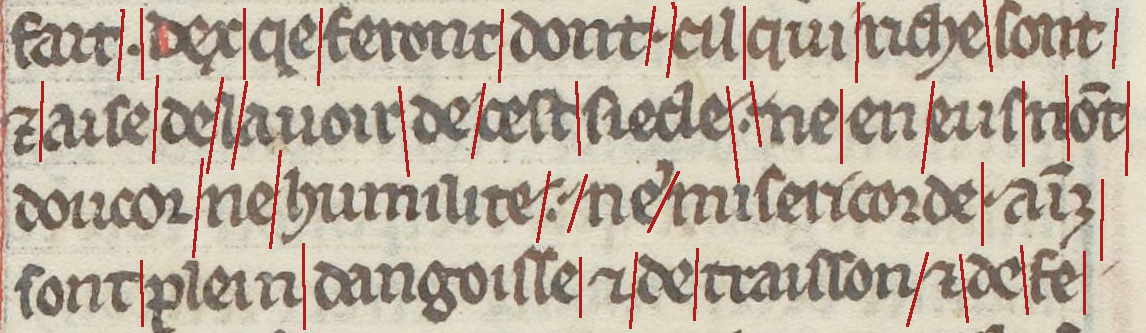
\includegraphics[width=\linewidth]{4-lines-p0215.png}

  \caption{ 4 lines from fol.103rb Manuscript fr. 412, Bibliothèque nationale de France.  Red lines indicate word boundaries}
  \label{fig:4lines}
\end{figure}

It must be stressed in this study that the difficulty inherent to segmentation is different for \textit{scripta continua} than the one for languages such as Chinese for which an already impressive amount of work has been. Chinese word segmentation has lately been driven by deep learning methods, specifically ones based on \textit{sequence to sequence translations}: \citet{chen2015long} defines a process based on LSTM model, while \citet{yu2019learning} uses BiDirectional GRU and CRF. \footnote{\citet{huang2019realistic} actually gave us the denomination used here: word boundary (WB) and word content (WC).}

Indeed, while the issue with Chinese seems to lie in the decomposition of relatively fixed characters, Old French or Medieval Latin present heavy variation of spelling. In \citet{camps_pandora}, Camps notes, in the same corpus, the existence of not less than 29 spellings of the word "\textit{cheval}" (horse in Old and Modern French) whose apparition counts span from 3907 to 1\footnote{These are \textit{cheval}, \textit{chevaus}, \textit{cheual}, \textit{ceval}, \textit{chevals}, \textit{cevaus}, \textit{chival}, \textit{ceual}, \textit{cheuaus}, \textit{cevals}, \textit{chaval}, \textit{chivaus}, \textit{chiual}, \textit{chevas}, \textit{cheuals}, \textit{chiuaus}, \textit{ceuaus}, \textit{chevaul}, \textit{chiuau}, \textit{chivals}, \textit{chevau}, \textit{kevaus}, \textit{chavaus}, \textit{cheuas}, \textit{keval}, \textit{cheua}, \textit{cheuau}, \textit{cheva}, \textit{chiuals}}. This  makes a dictionary-based approach rather difficult as it would rely on a high number of different spellings, making the computation highly complex.

\section{Description and evaluation}

\subsection{Architecture}

\subsubsection{Encoding of input and decoding}

The model is based on traditional text input encoding where each character is transcoded to an index. Output of the model is a mask that needs to be applied to the input: in the mask, characters are classified either as word boundary or word content (\textit{cf.} Table \ref{lst:input_output_example}.

\begin{table}[!ht]
\centering
\begin{tabular}{@{}ll@{}}
\hline
                       & \textbf{Sample}           \\  \hline
\textbf{Input  String} & \texttt{Ladamehaitees'enparti}     \\
\textbf{Mask   String} & \texttt{xSxxxSxxxxxSxxxSxxxxS}     \\
\textbf{Output String} & \texttt{La dame haitee s'en parti} \\ \hline
\end{tabular}
  \caption{Input, mask and human-readable output generated by the model. x are WC and S are WB}
  \label{lst:input_output_example}
\end{table}

For evaluation purposes, and to reduce the number of input classes, two options for data transcoding were used: a lower-case normalization and a "reduction to the ASCII character set" feature (fr. \ref{fig:normalization}). On this point, a lot of issues were encountered with transliteration of medieval paelographic characters that were part of the original datasets, as they are poorly interpreted by the \texttt{unidecode} python package. Indeed, \texttt{unidecode} will simply remove characters it does not understand. A derivative package named \texttt{mufidecode} was built for this reason(\citet{thibault_clerice_2019_3237731}): it takes precedent over \texttt{unidecode} equivalency tables when the data is known of the Medieval Unicode Font Initiative (MUFI, \citet{mufi}).

\begin{figure}[!ht]
  \centering
  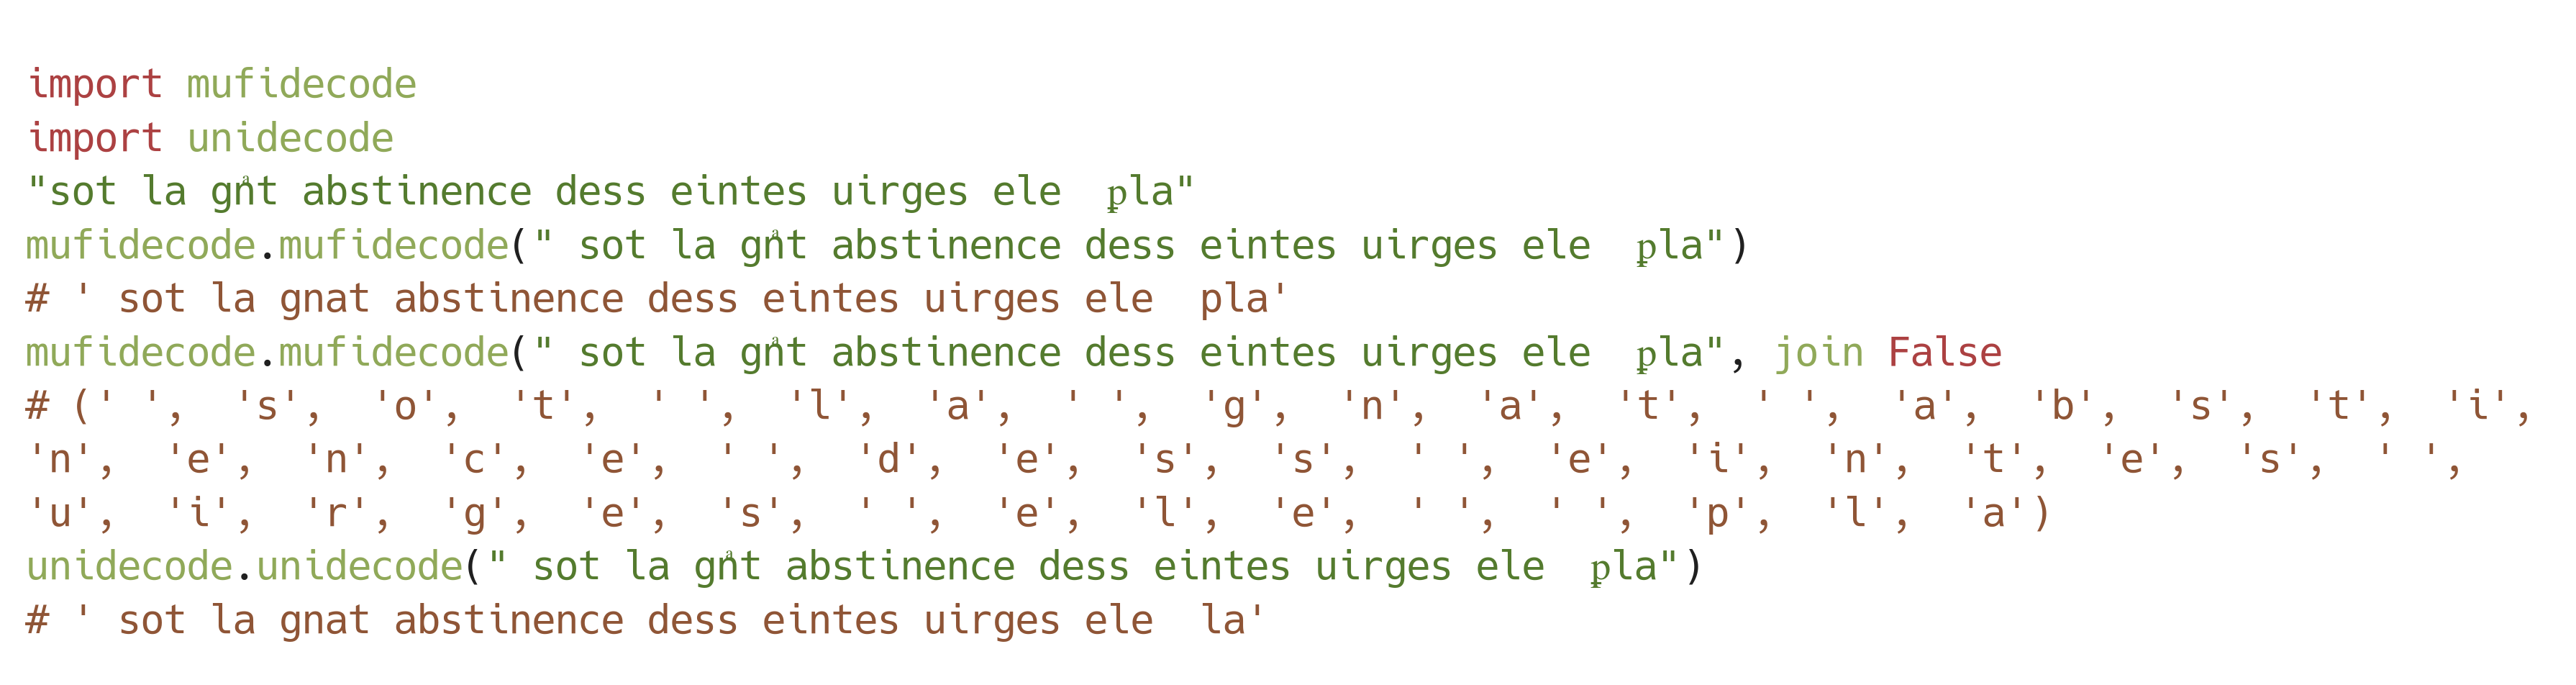
\includegraphics[width=\linewidth]{carbon.png}
  \caption{Different possibilities of pre-processing. The option with join=False was kept, as it keeps abbreviation marked as single characters. Note how \texttt{unidecode} loses the P WITH BAR}
  \label{fig:normalization}
\end{figure}

\subsubsection{Model}

Aside from normalizations of the input and output, three different model structures were tested. Every model is composed of one encoder, as described below, and one Linear Classifier which classifies into 5 classes : Start of Sentence (= SOS), End of Sentence (= EOS), Padding (= PAD), Masked Token (= Word Content), Space (= Word Boundary). For final scores, SOS, EOS and PAD were ignored.

The encoders are the following (configurations in parenthesis):

\begin{itemize}
  \item LSTM encoder with hidden cell (Embedding (512), Dropout(0.5), Hidden Dimension (512), Layers(10))
  \item Convolutional (CNN) encoder with position embeddings (Embedding (256), Embedding(Maximum Sentence Size=150), Kernel Size (5), Dropout(0.25), Layers (10))
  \item Convolutional (CNN) encoder without position embeddings (Embedding (256), Kernel Size (5), Dropout(0.25), Layers (10))
\end{itemize}

\subsection{Evaluation}

\subsubsection{Datasets}

The dataset is composed of transcriptions (from different projects) of manuscripts with unresolved abbreviation. The \textbf{Old French} is based on \citet{8269990}, \citet{pinche:hal-01628533}, \citet{jean_baptiste_camps_2019_2630574}, \citet{bfmmss}, and \citet{tnah_transcription}. It contains

\begin{itemize}
    \item 193,734 training examples;
    \item 23,581 validation examples;
    \item 25,512 test examples
    \item Number of classes in testing examples: 482,776 WC; 169,094 WB
    \item Number of classes in unknown examples: 26,393 WC; 10,193 WB
\end{itemize}

Examples were generated automatically. They are between 2 and 8 words-length. In order to recreate the condition of OCR noise, dots were added randomly (0.2) between words. In order to augment the dataset, words are randomly (0.1) passed over the next example\footnote{This data augmentation was limited to one word per sample}. If a minimum size of 7 characters was not met in the input sample, another word would be added to the chain, independently of the maximum number of words. The example however should not go beyond 100 characters. The results corpora should be varied in sizes as shown by Figure \ref{fig:word_sizes}. The corpora contains 193 different characters when not normalized, in which some MUFI characters appears few hundred times (\textit{cf.} Table \ref{tab:mufi_examples}).

\begin{figure}[!ht]
  \centering
  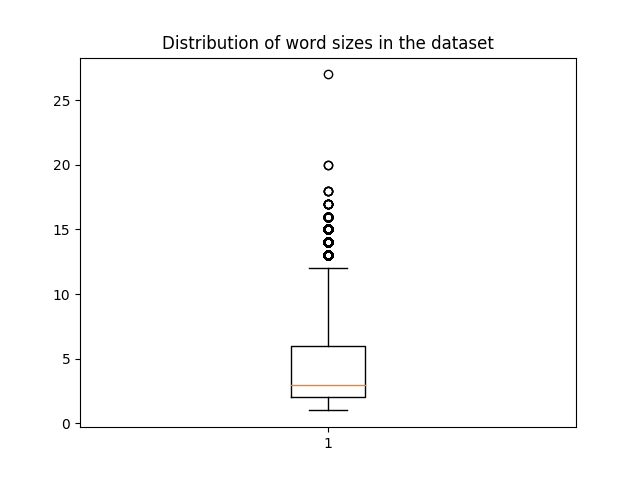
\includegraphics[width=\linewidth]{length.png}
  \caption{Distribution of word size over the train, dev and test corpora}
  \label{fig:word_sizes}
\end{figure}

\begin{table}[!ht]
\begin{tabular}{llll}
\hline
                                                   & Train dataset & Dev dataset & Test dataset \\ \hline
TIRONIAN SIGN ET                                   & 4367          & 541         & 539          \\
CON                             & 508           & 70          & 76           \\
P WITH STROKE THROUGH DESCENDER & 580           & 69          & 84           \\ \hline
\end{tabular}
  \caption{Examples of some MUFI characters distributions}
  \label{tab:mufi_examples}
\end{table}

\subsubsection{Results}

The training parameters were 0.00005 in learning rate for each CNN model, 0.001 for the LSTM model, and batch sizes of 64. Training reached a plateau fairly quickly for each model (\textit{cf.} \ref{fig:loss}). Each model except LSTM reached a really low loss and a high accuracy on the test set (\textit{cf.} \ref{tab:scores}). To compare the results, the \texttt{wordsegment} package \citet{WordSegment} was used as a baseline.

\begin{figure}[!ht]
  \begin{center}
    \begin{tikzpicture}
      \begin{axis}[
          width=\linewidth, % Scale the plot to \linewidth
          grid=major, 
          grid style={dashed,gray!30},
          xlabel=Epoch, % Set the labels
          ylabel=Accuracy,
          legend style={at={(0.5,-0.2)},anchor=north},
          x tick label style={rotate=90,anchor=east}
        ]
        \addplot table[x=Epoch,y=CNN 1,col sep=comma] {accuracies.csv}; 
        \addplot table[x=Epoch,y=CNN L,col sep=comma] {accuracies.csv}; 
        \addplot table[x=Epoch,y=CNN w/o P,col sep=comma] {accuracies.csv}; 
        \addplot table[x=Epoch,y=CNN N,col sep=comma] {accuracies.csv}; 
        \addplot table[x=Epoch,y=CNN L N,col sep=comma] {accuracies.csv}; 
        \addplot table[x=Epoch,y=LSTM,col sep=comma] {accuracies.csv}; 
        \legend{CNN, CNN L, CNN P, CNN N, CNN L N, LSTM}
      \end{axis}
    \end{tikzpicture}
    \caption{Training Loss (Cross-entropy) until plateau was reached. N = normalized, L = Lower, P = no position embedding. LSTM was removed as it did not go below 0.65}
  \label{fig:loss}
  \end{center}
\end{figure}

\begin{table}[!ht]
\centering
\begin{tabular}{lllllll}
\hline
Model    & Accuracy & Precision & Recall & FScore & WB FN & WB FP \\ \hline
Baseline & 0.989    & 0.986     & 0.984  & 0.985 & 4031 & 3229 \\
CNN      & 0.991    & 0.985     & 0.990  & 0.987 & 2137 & 3860 \\
CNN L    & 0.991    & 0.979     & 0.990  & 0.985 & \textbf{2117} & 3750 \\
CNN P    & \textbf{0.993}    & \textbf{0.990}& \textbf{0.991}  & \textbf{0.990} & 2432 & \textbf{2114} \\
CNN N    & 0.991    & 0.987     & 0.988  & 0.988 & 2756 & 3312 \\
CNN L N  & 0.992    & 0.988     & 0.989  & 0.988 & 2500 & 3567 \\
LSTM     & 0.939    & 0.637     & 0.918  & 0.720 & 21174 & 18662 \\ \hline
\end{tabular}
\caption{Scores over the test dataset. \\\hspace{\textwidth}For models: N = normalized, L = Lower, P = no position embedding. \\\hspace{\textwidth}In headers, FN = False Negative, FP = False Positive}
\label{tab:scores}
\end{table}

\subsubsection{Unknown texts}

While all models using CNN show improvement over the baseline, the models definitely do not significantly outperform (\textless 0.02 FScore). There is a reason for this: the baseline already performs nearly perfectly on the test corpus. The dictionary attack using n-grams did actually perform well. Therefore, an additional evaluation method was constructed. The baseline and the best achieving deep-learning model (CNN P) were evaluated on a secondary test corpus composed of texts that were not used in training: indeed, the training, dev and test corpus share the same texts while not sharing the same source corpora and as such the same writing, the same vocabulary. This new corpus is composed by 4 texts and counts 742 examples : the diplomatic edition of the \textit{Graal} (\citet{graal}), a \textit{Passion} and a \textit{Vie de Saint Leger}  (\citet{old_french_corpus}), a \textit{Vie de Saint Thibaut} (\citet{theobaldus}). Neither noise characters nor random keeping of words were applied.

The results here were highly different (\textit{cf.} Table \ref{tab:scores_unknown}): while it appears that the CNN is able to expand its "comprehension" of the language to newer texts, the new words are more difficult to take into account for the baseline \texttt{wordsegment} n-gram approach, resulting in a respective drop to 0.945 and 0.838 FScore. WordSegment specifically performed badly with WB false positives : it had 3658 over a corpus containing 10,193 WB token (around 35 \%).

\begin{table}[!ht]
\centering
\begin{tabular}{lllllll}
\hline
 & Accuracy & Precision & Recall & FScore & WB FN & WB FP \\ \hline
Baseline & 0.882 & 0.893 & 0.808 & 0.838 & 3658 & 644 \\
CNN P & \textbf{0.957} & \textbf{0.948} & \textbf{0.944} & \textbf{0.945} & \textbf{854} & \textbf{723} \\ \hline
\end{tabular}
\caption{Scores over the unknown dataset. FN = False Negative, FP = False Positive}
\label{tab:scores_unknown}
\end{table}

\subsubsection{Example of outputs}

The following inputs have been tagged with the CNN P model. Batches are constructed around the regular expression \texttt{\\W} with package \texttt{regex}. This explains why inputs such as \texttt{".i."} are automatically tagged as \texttt{" . i . "} by the tool. The input was stripped of its spaces before tagging, only the ground truth is shown for readability.

\begin{table}[!ht]
\centering
\begin{tabularx}{\textwidth}{|C|C|}
\hline
\textbf{Ground truth} & \textbf{Tokenized output} \\\hline
Aies joie et leesce en ton cuer car tu auras une fille qui aura .i. fil qui sera de molt grant merite devant Dieu et de grant los entre les homes.Conforte toi et soies liee car tu portes en ton ventre .i. fil qui son lieu aura devant Dieu et qui grant honnor fera a toz ses parenz. & Aies joie et leesce en ton cuer car tu auras une fille qui aura .  i .  fil qui sera de molt grant merite devant Dieu et de grant los entre les homes .  Confort e toi et soies liee car tu portes en ton ventre .  i .  fil qui son lieu aura devant Dieu et qui grant honnor fera a toz ses parenz .
\\\hline
\end{tabularx}
\caption{Output examples on a text from outside the dataset}
\label{tab:example_output}
\end{table}

\subsection{Evaluation on Latin data}

For the following evaluations, the same process was deployed: CNN without Position was evaluated against the baseline on both a test set composed by the same texts that the training text, and an unknown corpora composed by unseen texts.

\subsubsection{Latin Prose and Poetic Corpora}

\begin{table}[H]
\centering
\begin{tabular}{llllllll}
\hline
 & Corpus & Accuracy & Precision & Recall & FScore & WB FN & WB FP \\ \hline
Baseline & Test & 0.978 & 0.961 & 0.974 & 0.968 & 886 & 1893 \\
CNN P & Test & \textbf{0.992} & \textbf{0.987} & \textbf{0.989} & \textbf{0.988} & \textbf{439} & \textbf{584} \\ \hline
Baseline & Unknown & 0.933 & 0.897 & 0.890 & 0.893 & 1587 & 1409 \\
CNN P & Unknown & 0.970 & 0.952 & 0.956 & 0.954 & 600 & 709 \\ \hline
\end{tabular}
\caption{Scores over the Latin classical datasets. FN = False Negative, FP = False Positive}
\label{tab:latin_corpora}
\end{table}

The Latin data is much more noisy than the Old French, as it was less curated than the digital edition provided for Old French. They are part of the Perseus corpus \citet{perseus} and were cut into passages in the context of my thesis. The training, evaluation and test corpora are built upon prose works from Cicero and Suetonius. The unknown corpus is built upon \textit{Epigrammata} from Martial, from book 1 to book 2, as it should be fairly different in word order, vocabulary, etc. Both corpus were generated without noise and word keeping, with a maximum sample size of 150 characters.

\textbf{Statistics:}
\begin{itemize}
\item Number of training examples: 30725
\item Number of evaluation examples: 3558
\item Number of testing examples: 4406
\item Number of classes in testing examples: 105,915 WC; 26,404 WB
\item Number of classes in unknown examples: 35,910 WC; 8,828 WB
\end{itemize}

\textbf{Example:}

\begin{itemize}
    \item Input : operecuperemdeberemqueprofecto
    \item Output : opere cuperem deberemque profecto

\end{itemize}

\subsubsection{Medieval Latin corpora}

\begin{table}[H]
\centering
\begin{tabular}{llllllll}
\hline
 & Corpus & Accuracy & Precision & Recall & FScore & WB FN & WB FP \\ \hline
Baseline & Test & 0.989 & 0.981 & 0.986 & 0.982 & 1036 & 933 \\
CNN P & Test & \textbf{0.997} & \textbf{0.995} & \textbf{0.995} & \textbf{0.995} & \textbf{251} & \textbf{298} \\ \hline
Baseline & Unknown & 0.929 & 0.900 & 0.865 & 0.881 & 14,382 & 27,019 \\
CNN P & Unknown & 0.976 & 0.960 & 0.963 & 0.962 & 6509 & 7444\\ \hline
\end{tabular}
\caption{Scores over the Latin medieval datasets. FN = False Negative, FP = False Positive}
\label{tab:medieval_latin_corpora}
\end{table}

% test : 136,429+1036 WC / 933+33,120 WB
% unk  : 458,273+14,382 WC / 27,019+85,985 WB

The medieval Latin corpora is based on the project Formulae - Litterae - Chartae's open data (\citet{formulae}) for its training, evaluation and test sets; the unknown corpora is based on three texts from the Monumenta Germanica (\citet{germanica}) that are from early to late medieval period (Andreas Agnellus, Manegaldus, Theodoricus de Niem) and are drawn from the Corpus Corporum Project. Both corpus were generated without noise and word keeping, with a maximum sample size of 150 characters. The data presents some MUFI characters but still look like mostly normalized editions, unlike the Old French data.

\textbf{Statistics:}

\begin{itemize}
\item Number of training examples: 36814
\item Number of evaluation examples: 4098
\item Number of testing examples: 5612
\item Number of classes in testing examples: 137,465 WC; 34,053 WB
\item Number of classes in unknown examples: 472,655 WC; 113,004 WB
\end{itemize}p

\textbf{Example:}

\begin{itemize}
    \item Input : nonparvamremtibi	
    \item Output : non parvam rem tibi

\end{itemize}

\subsubsection{Latin epigraphic corpora}

\begin{table}[H]
\centering
\begin{tabular}{llllllll}
\hline
 & Corpus & Accuracy & Precision & Recall & FScore & WB FN & WB FP \\ \hline
Baseline & Test & 0.956 & 0.935 & 0.943 & 0.939 & 2646 & 3547 \\
CNN P & Test & \textbf{0.987} & \textbf{0.983} & \textbf{0.979} & \textbf{0.981} & \textbf{1149} & \textbf{722} \\ \hline
Baseline & Test Uppercase & 0.956 & 0.935 & 0.942 & 0.938 & 2664 & 3457 \\
CNN P & Test Uppercase & \textbf{0.979} & \textbf{0.972} & \textbf{0.967} & \textbf{0.969} & \textbf{1715} & \textbf{1275} \\ \hline
Baseline & Unknown & 0.879 & 0.834 & 0.817 & 0.825 & 8693 & 11332 \\
CNN P & Unknown & 0.953 & 0.939 & 0.926 & 0.932 & 4689 & 3112 \\ \hline
Baseline & Unknown Uppercase & 0.879 & 0.834 & 0.817 & 0.825 & 8693 & 11332 \\
CNN P & Unknown Uppercase & 0.936 & 0.914 & 0.902 & 0.908 & 6152 & 4464 \\ \hline
\end{tabular}
\caption{Scores over the Latin epigraphic datasets. FN = False Negative, FP = False Positive}
\label{tab:epigraphyc_latin}
\end{table}

% test : 136,429+1036 WC / 933+33,120 WB
% unk  : 458,273+14,382 WC / 27,019+85,985 WB

The epigraphic Latin corpora is based on the Epigraphic Database Heidelberg open data \citet{formulae} for its training, evaluation and test sets (HD000001-HD010000 and HD010001-HD020000 from \citet{edh}) while the corpus of unknown is drawn from an automatic conversion of the Pompei Inscriptions (\citet{pompei}). Both the baseline and the model were evaluated on uppercase data, as it would normally be the state the text would be found in. Each of the corpora presents a high number of unresolved abbreviations (\textit{ie.} one letter words). Both corpus were generated without noise and word keeping, with a maximum sample size of 150 characters. The data presents some polytonic Greek characters, some sample being only in Greek.

\textbf{Statistics:}

\begin{itemize}
\item Number of training examples: 46,423
\item Number of evaluation examples: 5,802
\item Number of testing examples: 5,804
\item Number of classes in testing examples: 107,963 WC; 31,900 WB
\item Number of classes in unknown examples: 127,268 WC; 38,055 WB
\end{itemize}

\textbf{Example:}

\begin{itemize}
    \item Input : DnFlClIuliani	
    \item Output : D n Fl Cl Iuliani
\end{itemize}

\subsection{Discussion}

Aside from a graphical challenge, word segmentation in OCR from manuscripts can actually be treated as a NLP task. Word segmentation for some text can be even difficult for humanist, as shown by the manuscript sample, and as such, it seems that the post-processing of OCR through tools like this one can be a better way to achieve data-mining of raw datasets.

The negligible effects of the different normalization methods (lower-casing; ASCII reduction; both) were surprising. The presence of certain MUFI characters might provide enough information about segmentation and be of sufficient quantity for them not to impact the network weights. 

While the baseline performed unexpectedly well on the test corpus, the CNN model definitely performed better on a completely unknown corpus. In this context, the proposed model actually shows its ability to carry over unknown corpora in a better way than classical n-gram approaches. In light of the high accuracy of the CNN model, the model should perform the same way independently of the language in Medieval Western Europe,.

\subsection{Conclusion}

Achieving 0.99 accuracy on word segmentation with a corpus as large as 25,000 test samples seems to be the first step for a more thorough data mining of OCRed manuscript. Given the results, studying the importance of normalization and lowering should probably be a further step, as it might be of high influence in smaller corpora. 

\subsection{Acknowledgements}

Boudams has been made possible by two open-source repositories from which I learned and copied bits of implementation of certain modules and without which none of this paper would have been possible: \citet{enrique_manjavacas_2019_2654987} and \citet{bentrevett}. This tool was originally intended for post-processing OCR for the presentation \citet{pinchecampsclerice} at DH2019 in Utrecht.



\bibliographystyle{plainnat}
\bibliography{article}

\appendix\footnotesize

\section{Annex 1 : Confusion of CNN without position embeddings}

\begin{figure}[H]
  \centering
  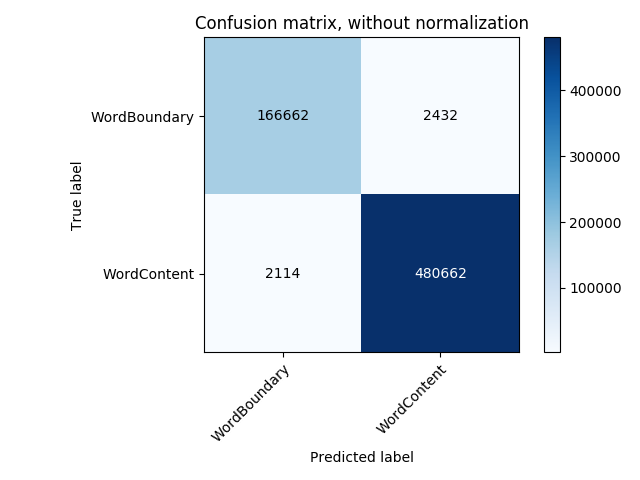
\includegraphics[width=\linewidth]{confusion.png}
  \caption{Confusion matrix of the CNN model without position embedding}
  \label{fig:confusion_matrix}
\end{figure}

\end{document}